\documentclass[10pt,a4paper]{report}
%\usepackage[utf8]{inputenc}
\usepackage[latin1]{inputenc}
\usepackage{amsmath}
\usepackage{amsfonts}
\usepackage{amssymb}
\usepackage{multicol, blindtext}
\usepackage{textcomp}
\usepackage{graphicx}
\usepackage{lipsum}
\usepackage{mathtools}

\title{Transformada de Fourier}

\begin{document}



%\title{Medi��o de Velocidade usando um Sensor de Luminosidade}

\author{Danilo Souza, Hugo Santos, Welton Ara�jo}
%Matr\'iculas: 10080000801, 10080000701, 10080000501}
%\thanks{Engenharia da Computa\c{c}\~ao, Universidade Federal do Par\'a, Bel\'em-PA, Brasil}
\maketitle

%Emails: \{dhcsouza, huggosan, weltonmaxx007\}@gmail.com\\

\section{Funcionamento}
O c�digo mostra o c�lculo da transformada de fourier de: \begin{equation}
e^-(2t)u(t)
\end{equation} � necess�rio, para o c�digo, que se calcule os valores de T0 e Ts. Os valores usados s�o Ts = 1/64 e T0 = 4. Assim N0 fica igual a 256 amostras.

\section{Resultados}
Se os valores de T0 e Ts forem modificados, o sinal perde a caracter�stica que realmente deveria ter, se o Ts for aumentado deixando o T0 constante o sinal perde a caracteristica de exponencial e passa a ter o formato de um polin�mio de segundo grau. Com o T0 sendo aumentado e o Ts mantido constante a exponencial convergir� rapidamente. Os dois elementos variados aumenta o n�mero de amostrar N0 mas apenas o Ts esta diretamente ligado ao sinal usado na transformada e por isso acaba mudando a caracter�stica do mesmo.

%\begin{multicols}{1}
\begin{figure}[h]
	\centering
	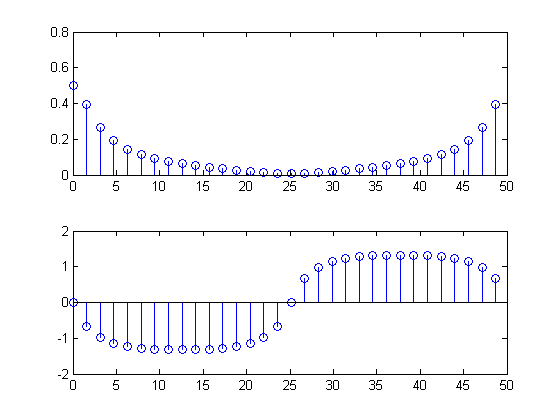
\includegraphics[scale=0.25]{./pictures/cap3grafico1.png}
	\caption{ Ts =1/8, T0 = 4}
	%\label{fig:semSolucao1}
\end{figure}
\begin{figure}[h]
	\centering
	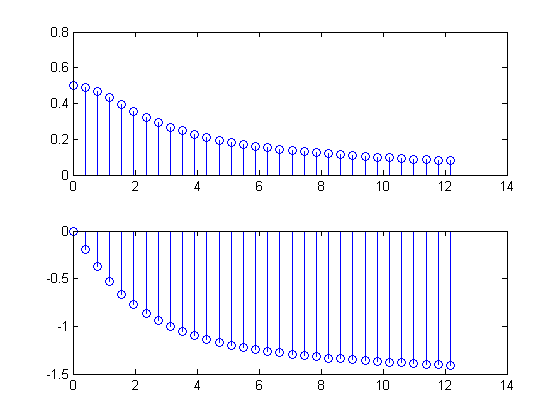
\includegraphics[scale=0.25]{./pictures/cap3grafico2.png}
	\caption{ Ts = 1/64, N0 = 16}
	%\label{fig:semSolucao2}
\end{figure}
\begin{figure}[h]
	\centering
	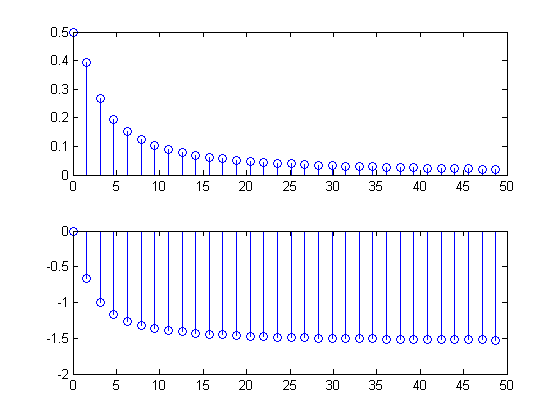
\includegraphics[scale=0.25]{./pictures/cap3grafico3.png}
	\caption{Ts=1/64, T0=4}
	%\label{fig:semSolucao4}
\end{figure}
%\end{multicols}
\end{document}